
\documentclass[a4paper,11pt]{article}
\usepackage[utf8]{inputenc}
\usepackage[T1]{fontenc}
\usepackage[swedish]{babel}
\usepackage{amsmath,amssymb,amsfonts}
\usepackage{graphicx}
\usepackage{enumitem}
\usepackage{geometry}
\usepackage{tikz}
\geometry{margin=2.5cm}

\title{Repetitionsuppgifter -- Matematik 2b}
\author{Fabian Tingstrand}
\date{\today}

\begin{document}

\maketitle

\section{Analys av andragradsfunktioner}

\begin{enumerate}[label=\textbf{\arabic*.}]
    \item För funktionen $f(x) = x^2 - 6x + 5$:
    \begin{enumerate}[label=\alph*)]
        \item Bestäm funktionens nollställen
        \item Bestäm symmetrilinjen
        \item Bestäm extrempunkten och avgör om det är ett maximum eller minimum
    \end{enumerate}
    
    \item Nedan visas grafen till en andragradsfunktion $f(x) = ax^2 + bx + c$:
    
    \begin{center}
    \begin{tikzpicture}[scale=0.7]
        \draw[->] (-3,0) -- (4,0) node[right] {$x$};
        \draw[->] (0,-1) -- (0,5) node[above] {$y$};
        \foreach \x in {-2,-1,1,2,3}
            \draw (\x,0.1) -- (\x,-0.1) node[below] {$\x$};
        \foreach \y in {1,2,3,4}
            \draw (0.1,\y) -- (-0.1,\y) node[left] {$\y$};
        \draw[thick, domain=-1.5:3.5, smooth, variable=\x, blue] plot ({\x}, {-\x*\x+2*\x+3});
    \end{tikzpicture}
    \end{center}
    
    \begin{enumerate}[label=\alph*)]
        \item Bestäm funktionens nollställen
        \item Bestäm symmetrilinjen
        \item Bestäm funktionsuttrycket $f(x) = ax^2 + bx + c$
    \end{enumerate}

    \item För funktionen $f(x) = 3x^2 + 6x - 2$:
    \begin{enumerate}[label=\alph*)]
        \item Bestäm funktionens nollställen
        \item Bestäm symmetrilinjen
        \item Bestäm extrempunkten och avgör om det är ett maximum eller minimum
    \end{enumerate}
    
    \item För funktionen $f(x) = -x^2 + 4x + 5$:
    \begin{enumerate}[label=\alph*)]
        \item Bestäm funktionens nollställen
        \item Bestäm symmetrilinjen
        \item Bestäm extrempunkten och avgör om det är ett maximum eller minimum
    \end{enumerate}
    \break
    \item Nedan visas grafen till en andragradsfunktion $f(x) = ax^2 + bx + c$:
    
    \begin{center}
    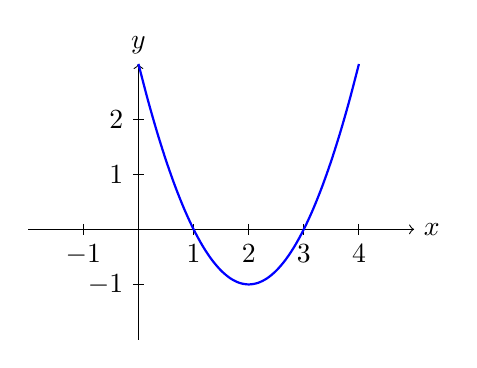
\begin{tikzpicture}[scale=0.7]
        \draw[->] (-2,0) -- (5,0) node[right] {$x$};
        \draw[->] (0,-2) -- (0,3) node[above] {$y$};
        \foreach \x in {-1,1,2,3,4}
            \draw (\x,0.1) -- (\x,-0.1) node[below] {$\x$};
        \foreach \y in {-1,1,2}
            \draw (0.1,\y) -- (-0.1,\y) node[left] {$\y$};
        \draw[thick, domain=0:4, smooth, variable=\x, blue] plot ({\x}, {\x*\x-4*\x+3});
    \end{tikzpicture}
    \end{center}
    
    \begin{enumerate}[label=\alph*)]
        \item Bestäm funktionens nollställen
        \item Bestäm symmetrilinjen
        \item Bestäm funktionsuttrycket $f(x) = ax^2 + bx + c$
    \end{enumerate}
    
    \item Givet är att en andragradsfunktion $f(x)$ har nollställena $x = -2$ och $x = 3$, och att $f(0) = -6$.
    \begin{enumerate}[label=\alph*)]
        \item Bestäm funktionsuttrycket $f(x) = ax^2 + bx + c$
        \item Bestäm symmetrilinjen
        \item Bestäm extrempunkten och avgör om det är ett maximum eller minimum
    \end{enumerate}
    
    \item Givet är att en andragradsfunktion $f(x) = ax^2 + bx + c$ har en extrempunkt i $(1, -4)$ och att grafen skär $y$-axeln i punkten $(0, 2)$.
    \begin{enumerate}[label=\alph*)]
        \item Bestäm funktionsuttrycket $f(x) = ax^2 + bx + c$
        \item Bestäm funktionens nollställen
        \item Bestäm symmetrilinjen
    \end{enumerate}
\end{enumerate}

\section{Problemlösning med andragradsfunktioner}

\begin{enumerate}[label=\textbf{\arabic*.}]
    \item En boll kastas rakt uppåt från marken med en utgångshastighet på $20$ m/s. Bollens höjd $h$ (i meter) efter $t$ sekunder ges av funktionen $h(t) = 20t - 5t^2$. 
    \begin{enumerate}[label=\alph*)]
        \item När når bollen sin högsta höjd?
        \item Hur hög når bollen som högst?
        \item När träffar bollen marken igen?
    \end{enumerate}
    
    \item En rektangel har omkretsen $24$ cm. Låt $x$ vara rektangelns bredd.
    \begin{enumerate}[label=\alph*)]
        \item Uttryck rektangelns längd som en funktion av $x$.
        \item Uttryck rektangelns area $A$ som en funktion av $x$.
        \item Vilka värden kan $x$ anta?
        \item För vilket värde på $x$ blir arean maximal?
        \item Vad är den maximala arean?
    \end{enumerate}
\end{enumerate}

% \section{Blandade uppgifter}
% 
% \begin{enumerate}[label=\textbf{\arabic*.}]
%     \item Bestäm $a$ så att funktionen $f(x) = x^2 + ax + 4$ har sitt minimum i punkten $(2, -5)$.
%     
%     \item Bestäm $k$ så att funktionen $f(x) = kx^2 - 4x + 3$ har sitt maximum i punkten $(1, 0)$.
%     
%     \item Funktionen $f(x) = ax^2 + bx + c$ har nollställena $x = -3$ och $x = 2$, och $f(0) = -6$. Bestäm konstanterna $a$, $b$ och $c$.
%     
%     \item Funktionen $f(x) = x^2 + bx + c$ har en extrempunkt i $(2, -1)$. Bestäm konstanterna $b$ och $c$.
%     
%     \item En andragradsfunktion $f(x) = ax^2 + bx + c$ har nollställena $x = -1$ och $x = 3$, och grafen till funktionen går genom punkten $(1, -4)$. Bestäm funktionsuttrycket.
%     
%     \item En andragradsfunktion $f(x) = ax^2 + bx + c$ har en extrempunkt i $(2, 3)$ och grafen skär $y$-axeln i punkten $(0, -1)$. Bestäm funktionsuttrycket.
%     
%     \item Grafen till en andragradsfunktion $f(x) = ax^2 + bx + c$ går genom punkterna $(-1, 0)$, $(2, 0)$ och $(0, -2)$. Bestäm funktionsuttrycket.
%     
%     \item Bestäm alla värden på $m$ för vilka ekvationen $x^2 - mx + m = 0$ har reella lösningar.
%     
%     \item Bestäm alla värden på $k$ för vilka funktionen $f(x) = x^2 + kx + 9$ har sitt minimum för ett negativt $x$-värde.
%     
%     \item Bestäm alla värden på $p$ för vilka funktionen $f(x) = x^2 + px + p$ har sitt minimum på $y$-axeln.
% \end{enumerate}

\end{document}